\documentclass[border=3pt]{standalone}
% Preâmbulo compartilhado pelos diagramas TikZ da aula 4 de Navegação (Representação de Mapas)
\usepackage[T1]{fontenc}
\usepackage[utf8]{inputenc}
\usepackage{lmodern}
\usepackage{amsmath}
\usepackage{xcolor}
\usepackage{tikz}
\usetikzlibrary{arrows.meta,angles,quotes,decorations.pathmorphing,decorations.pathreplacing,calc,
                positioning,shapes.geometric,shapes.misc,backgrounds,fit,
                math}

% Paleta (mesma dos SVGs originais)
\definecolor{dblue}{HTML}{2A5B8C}
\definecolor{dorange}{HTML}{B3541E}
\definecolor{dgreen}{HTML}{4A7C59}
\definecolor{dred}{HTML}{9C4B4B}
\definecolor{dcream}{HTML}{F4F1EA}
\definecolor{dshade}{HTML}{DDD7C9}

% Função gaussiana (não normalizada por padrão de escala visual)
\pgfmathdeclarefunction{gauss}{3}{%
  \pgfmathparse{1/(#3*sqrt(2*pi))*exp(-((#1-#2)^2)/(2*#3^2))}%
}

% Estilos comuns (prefixo d... para não colidir com chaves internas do pgf)
\tikzset{
  >={Stealth[length=2mm]},
  dguide/.style={gray!55, dashed, line width=0.4pt},
  daxis/.style={gray!60, line width=0.7pt, ->},
  dbody/.style={fill=black!3, draw=black!80, line width=1pt},
  dacc/.style={draw=dblue, line width=1pt},
  dlbl/.style={black!55, font=\small},
  dsub/.style={black!45, font=\footnotesize},
  dstate/.style={circle, draw=black!80, fill=dcream, line width=1pt,
                 minimum size=17mm, font=\large, inner sep=1pt},
  dobs/.style={circle, draw=black!80, fill=dshade, line width=1pt,
               minimum size=14mm, font=\large, inner sep=1pt},
  dbox/.style={rounded corners=2pt, draw=black!80, fill=dcream, line width=1pt,
               align=center, inner sep=6pt},
  dop/.style={circle, draw=black!80, fill=white, line width=1pt,
              minimum size=6mm, inner sep=0pt, font=\small},
  dtrans/.style={->, dblue, line width=1pt},
  dmeas/.style={->, dorange, line width=1pt},
  dcurve/.style={line width=1pt, dblue},
  dcurveb/.style={line width=1.4pt, dorange},
}

\begin{document}
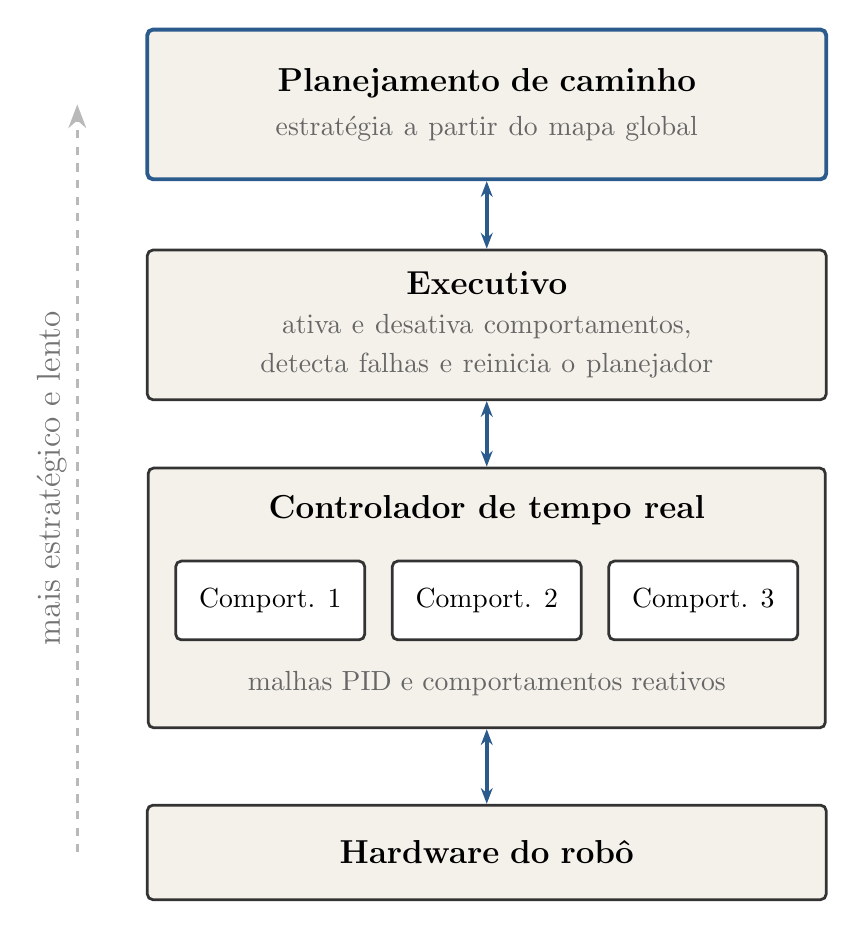
\begin{tikzpicture}[x=1cm,y=1cm]

  \tikzset{lay/.style={dbox, minimum width=8.6cm, text width=8.2cm, align=center, font=\large}}

  \node[lay, draw=dblue, line width=1.4pt, minimum height=1.9cm] (p) at (0,8.6)
    {\textbf{Planejamento de caminho}\\[2pt]{\normalsize\color{black!60}estratégia a partir do mapa global}};
  \node[lay, minimum height=1.9cm] (e) at (0,5.8)
    {\textbf{Executivo}\\[2pt]{\normalsize\color{black!60}ativa e desativa comportamentos,\\detecta falhas e reinicia o planejador}};

  % controlador de tempo real com comportamentos
  \node[dbox, minimum width=8.6cm, minimum height=3.3cm, anchor=north] (c) at (0,4.0) {};
  \node[font=\large\bfseries] at (0,3.45) {Controlador de tempo real};
  \foreach \x/\t in {-2.75/Comport. 1, 0/Comport. 2, 2.75/Comport. 3} {
    \node[dbox, minimum width=2.4cm, minimum height=1.0cm, align=center, font=\normalsize, fill=white] at (\x,2.3) {\t};
  }
  \node[font=\normalsize, black!60] at (0,1.25) {malhas PID e comportamentos reativos};

  \node[lay, minimum height=1.2cm] (h) at (0,-0.9) {\textbf{Hardware do robô}};

  \draw[dtrans, line width=1.3pt, <->] (p.south) -- (e.north);
  \draw[dtrans, line width=1.3pt, <->] (e.south) -- (c.north);
  \draw[dtrans, line width=1.3pt, <->] (c.south) -- (h.north);

  \draw[dguide, line width=1.2pt, -{Stealth[length=3mm]}] (-5.2,-0.9) -- (-5.2,8.6) node[midway, sloped, above, dlbl, font=\large] {mais estratégico e lento};

\end{tikzpicture}
\end{document}
